\section{Question 3}

\subsection{Jacobi}
% TODO comparer itérations
On remarque tout d'abord à l'aide de la figure~\ref{fig:arj}
et de la figure~\ref{fig:rhoj} que pour $a \geq 0.25$,
Jacobi ne converge pas pour tout $r$ mais uniquement à partir
d'un certain $r$.

Le $r$ pour lequel Jacobi commence à converge correspond d'ailleurs
assez bien au point où le rayon spectral passe en dessous de 1.

La figure~\ref{fig:rhoj} nous montre que le rayon spectral est
décroisant en fonction de $r$ ce qui nous invite à penser que
la convergence sera de plus en plus rapide mais ça ne nous
dit rien sur l'évolution de l'erreur.

La figure~\ref{fig:arj} nous donne un aperçu de l'impact de $r$
sur l'erreur pour différentes valeurs de $a$.
On voit qu'en choisissant correctement $r$ on a une erreur semblable
pour $a \leq 0.25$ mais pour $a \geq 0.3$, on a une nette
diminution de l'erreur.
Pour $a = 0.45$ (pas représenta sur la figure~\ref{fig:rhoj}),
l'erreur était de 7000 mais avec la régularisation, on obtenait
1500.

On voit que pour $a \geq 0.3$, la régularisation donne de meilleurs résultats
pour autant qu'on choisissse un bon $r$.
Pour $a \leq 0.25$ par contre, la régularisation donne de moins bons résultats.

On a d'ailleurs pas toujours la convergence pour $a \geq 0.25$ mais à partir
d'un certain $r$, ça converge.
Le meilleur $r$ pour $a \geq 0.3$ semble être le premier $r$ à partir duquel
ça converge.
Pour $a \leq 0.25$, ça n'a pas l'air aussi simple mais la fonction semble
unimodale donc on peut aisément trouver le $r$ qui minimise l'erreur.

\subsection{Gauss-Seidel}
La figure~\ref{fig:rhogs} nous invite à penser que pour
$a < 0.5$, le rayon spectral est plus petit que 1.
On voit d'ailleurs avec la figure~\ref{fig:args} que contrairement
à Jacobi, on a pas de problème de convergence.

On a aussi une erreur semblable pour un $r$ bien choisi
avec et sans la régularisation pour $a \leq 0.25$ et une nette
diminution pour $a \geq 0.3$.

La fonction de l'erreur en fonction de $r$ semble à nouveau unimodale
ce qui nous permettra d'effectuer une recherche unimodale.

\subsection{Comparaison entre Gauss-Seidel et Jacobi}
En comparant la figure~\ref{fig:arj} et la figure~\ref{fig:args}, on voit
que lorsque Jacobi converge, ils ont la même erreur.
Seulement, Jacobi ne converge pas toujours pour le meilleur $r$ pour Gauss-Seidel.
C'est d'ailleurs assez naturel qu'ils aient la même erreur car ils résolvent le même
système linéaire.
C'est donc pour ça qu'on a pas comparé l'erreur à la question 2.


\begin{table}
  \centering
  \begin{tabular}{|l|l|l|l|l|l|}
    \hline
    \multirow{2}{*}{$a$} & \multirow{2}{*}{$r$} & \multicolumn{2}{l|}{Jacobi} & \multicolumn{2}{l|}{Gauss-Seidel}\\
    \cline{3-6}
      &  & $i_1$ & $i_2$ & $i_1$ & $i_2$\\
    \hline
    \multirow{3}{*}{$0.1$} & 0.1 & 20 & 20 & 12 & 12 \\
    \cline{2-6}
      & 0.2 & 21 & 21 & 12 & 12 \\
      \cline{2-6}
      & 0.3 & 21 & 21 & 12 & 12 \\
    \hline
    \multirow{3}{*}{$0.2$} & 0.1 & 79 & 79 & 24 & 24 \\
    \cline{2-6}
      & 0.2 & 69 & 69 & 21 & 22 \\
      \cline{2-6}
      & 0.3 & 56 & 56 & 19 & 19 \\
    \hline
    \multirow{3}{*}{$0.25$} & 0.1 & 500 & 500 & 34 & 34 \\
    \cline{2-6}
      & 0.2 & 244 & 244 & 29 & 29 \\
      \cline{2-6}
      & 0.3 & 119 & 119 & 24 & 24\\
    \hline
    \multirow{3}{*}{$0.3$} & 0.1 & 500 & 500 & 50 & 52 \\
    \cline{2-6}
      & 0.2 & 500 & 500 & 38 & 39 \\
      \cline{2-6}
      & 0.3 & 500 & 500 & 29 & 29 \\
      \hline
      \multirow{3}{*}{$0.4$} & 0.1 & 500 & 500 & 135 & 144 \\
    \cline{2-6}
      & 0.2 & 500 & 500 & 64 & 66 \\
      \cline{2-6}
      & 0.3 & 500 & 500 & 38 & 39 \\
      \hline
  \end{tabular}
  \caption{Nombre d'itération nécessaire pour que l'itération se termine (soit pour des valeurs $<500$ si cela converge, soit pour 500 qui est le nombre d'itérations maximales de l'algorithme) pour différentes valeurs de $a$ et de $r$.
  $i_1$ est le nombre d'itérations pour le premier système et $i_2$ pour le deuxième.}
  \label{tab:iterQ3JvsGS}
\end{table}


\begin{figure}
  \centering
  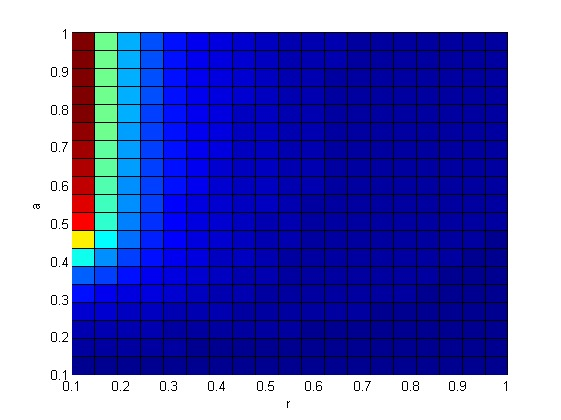
\includegraphics[width=11cm]{convergence_JacobiQ3.png}
  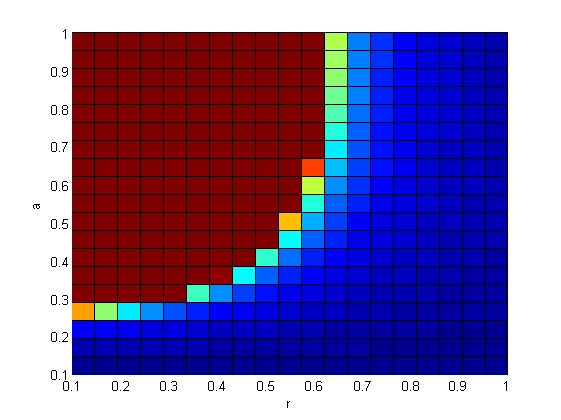
\includegraphics[width=11cm]{convergence_GSQ3.png}
  \caption{Graphes représentant les valeurs de $i_1$, le nombre d'itération nécessaires  pour différentes valeurs de a et de r, pour les méthode de Jacobi (graphe du haut) et de Gauss-Seidel (graphe du bas). Le rouge étant une zone de non-convergence (nombre d'itération vaut 500) et le bleu une convergence rapide (a titre d'exemple, la case du bas à droite vaut respectivement 10 pour Jacobi et 14 pour Gauss-Seidel).}
  \label{fig:JvsGS}
\end{figure}

Comme on peut le remarquer dans le tableau \ref{tab:iterQ3JvsGS} ou sur les graphes de la figure \ref{fig:JvsGS}, les deux méthodes ont tendance à converger plus rapidement pour des petites valeurs de $a$ et pour des  grandes valeurs de $r$. Gauss-Seidel présente toujours un net avantage sur Jacobi en ce qui concerne la vitesse de convergence mais aussi la zone de convergence. En effet, à la question 2, nous avions $\rho (\mathcal{G}) = (\rho (\mathcal{J}))^2$, et ainsi les méthodes de Jacobi et de Gauss-Seidel convergeaient et divergeaient en même temps. Ici ce n'est plus le cas.



\subsection{Analyse du rayon spectral}

Comme illustré aux figures \ref{fig:rhoj} et \ref{fig:rhogs}, le rayon spectral tend à diminuer pour un $r$ de plus en plus grand. On constate également que la méthode de la question 3 n'a un rayon spectral plus petit qu'à la question 2 qu'à partir d'un certain $r$.
La régularisation n'est donc intéressante au point de vue de la vitesse qu'à partir d'un certain $r$. Par exemple pour $a = 0.3$, il faut choisir un minimum de $r = 0.5$ pour que la méthode de Gauss-Seidel converge plus rapidement.

\begin{figure}
  \centering
  \begin{subfigure}[b]{0.45\textwidth}
    \includegraphics[width=\textwidth]{Q3/arJacobi.png}
    \caption{Erreur pour différents $a$ en fonction de $r$ de Jacobi.
      Lorsque la méthode ne converge pas, le point n'est pas représenté.
      L'erreur est calculée comme la norme de Frobenius entre l'image de départ
      et l'image défloutée. Les croix représentent quant à elles l'erreur obtenue pour différent a à la question 2 (identique pour Jacobi et Gauss-Seidel).}
    \label{fig:arj}
  \end{subfigure}%
  ~
  \begin{subfigure}[b]{0.45\textwidth}
    \includegraphics[width=\textwidth]{Q3/arGauss-Seidel.png}
    \caption{Erreur pour différents $a$ en fonction de $r$ de Gauss-Seidel.
      Lorsque la méthode ne converge pas, le point n'est pas représenté.
      L'erreur est calculée comme la norme de Frobenius entre l'image de départ
      et l'image défloutée. Les croix représentent quant à elles l'erreur obtenue pour différent a à la question 2 (identique pour Jacobi et Gauss-Seidel).}
    \label{fig:args}
  \end{subfigure}

  \begin{subfigure}[b]{0.45\textwidth}
    \includegraphics[width=\textwidth]{Q3/rhoJacobi.png}
    \caption{Graphe du rayon spectral de A $\rho(A)$ en fonction de r et ce pour différentes valeurs de a pour la méthode de Jacobi. Les croix indiquent quant à elles les valeurs du rayon spectral obtenues à la question 2.}
    \label{fig:rhoj}
  \end{subfigure}%
  ~
  \begin{subfigure}[b]{0.45\textwidth}
    \includegraphics[width=\textwidth]{Q3/rhoGauss-Seidel.png}
    \caption{Graphe du rayon spectral de A $\rho(A)$ en fonction de r et ce pour différentes valeurs de a pour la méthode de Gauss-Seidel. Les croix indiquent quant à elles les valeurs du rayon spectral obtenues à la question 2.}
    \label{fig:rhogs}
  \end{subfigure}
  \caption{Graphes sur le rayon spectral et l'erreur.}
  \label{fig:arrho}
\end{figure}

\subsection{Recherche unimodale}
Bien qu'on pourrait faire une recherche unimodale directement, on prenant
$+\infty$ comme erreur par convention quand ça ne converge pas,
commençons par faire une recherche binaire pour trouver à partir de quel
$r$ ça converge.

Faisons ensuite une recherche unimodale du minimum
avec $r$ entre cette valeur et 0.5.
En effet, comme vu à la figure~\ref{fig:arj} et à la figure~\ref{fig:args},
le minimum se situe toujours entre 0 et 0.5.

On obtient la figure~\ref{fig:best} où on observe les même minimums que sur la figure~\ref{fig:arj}
et la figure~\ref{fig:args}.
On voit que la valeur de $r$ est à peu prêt la même pour Gauss-Seidel et Jacobi,
c'est normal car leur erreur en fonction de $r$ est pareil comme ils résolvent le même système.
Ce n'est par contre plus le cas pour $a \geq 0.25$ car Jacobi ne converge alors plus pour tout $r$.
Dans ce cas, le minimum est atteint pour le premier $r$ tel qu'il converge.

\begin{figure}
  \centering
  \includegraphics[width=\textwidth]{Q3/best.png}
  \caption{Valeur de $r$ donnant la plus petite erreur pour différentes valeurs de $a$.}
  \label{fig:best}
\end{figure}
